\documentclass{beamer}
\usepackage[T1]{fontenc}
\usepackage[utf8]{inputenc}
\usepackage{hyperref,lmodern}
\usepackage[spanish]{babel}
\mode<presentation>
{
  \usetheme{Warsaw}
  
  \setbeamercovered{transparent}
  
}

\usepackage{times}

\title{Estructuraci\'on de una unidad did\'actica: Uso del software libre}

\author{Germán Darío Avendaño Ramírez}
% - Use the \inst{?} command only if the authors have different
%   affiliation.

\institute[Universities of Somewhere and Elsewhere] 
{
  \inst{}%
  Área de Matemáticas\\
  I.E.D. Arborizadora Baja
  }
% - Use the \inst command only if there are several affiliations.
% - Keep it simple, no one is interested in your street address.

\date{20 de julio de 2017}

\subject{Talks}

% If you have a file called "university-logo-filename.xxx", where xxx
% is a graphic format that can be processed by latex or pdflatex,
% resp., then you can add a logo as follows:

\pgfdeclareimage[height=0.5cm]{university-logo}{logo-colegio.png}
\logo{\pgfuseimage{university-logo}}



% Delete this, if you do not want the table of contents to pop up at
% the beginning of each subsection:

% If you wish to uncover everything in a step-wise fashion, uncomment
% the following command: 

%\beamerdefaultoverlayspecification{<+->}
\hyphenation{Contextua-lización}

\begin{document}

\begin{frame}
  \titlepage
\end{frame}

\begin{frame}{``No hay animal tan manso que atado no se irrite''}
  \tableofcontents
  % You might wish to add the option [pausesections]
\end{frame}


% Since this a solution template for a generic talk, very little can
% be said about how it should be structured. However, the talk length
% of between 15min and 45min and the theme suggest that you stick to
% the following rules:  

% - Exactly two or three sections (other than the summary).
% - At *most* three subsections per section.
% - Talk about 30s to 2min per frame. So there should be between about
%   15 and 30 frames, all told.
\begin{frame}{Contextualización}
\begin{itemize}
\item Esta presentación se hizo en una jornada pedagógica en el año 2012 y hace parte de un proyecto que inicié en el año 2011, creando una plataforma virtual basada en el software libre Chamilo LMS (Learning Management System) y que fue utilizada por estudiantes de grado noveno y once. Posteriormente se usó en el año 2012 y 2013 también con estudiantes de diferentes grados.  
\item La evaluación de la experiencia fue satisfactoria aunque hubo inconvenientes con el servidor, el cual fue gratuito y por lo tanto los servicios fueron muy limitados. Cuando se conectaban simultáneamente más de 100 estudiantes se caía la plataforma.
\end{itemize}
\end{frame}
\begin{frame}
Planteo nuevamente el proyecto, ésta vez si solicitando presupuesto, para hacernos a un servidor de pago que nos ofrezca una buena capacidad, para que puedan conectarse simultáneamente cientos de estudiantes.
\begin{center}
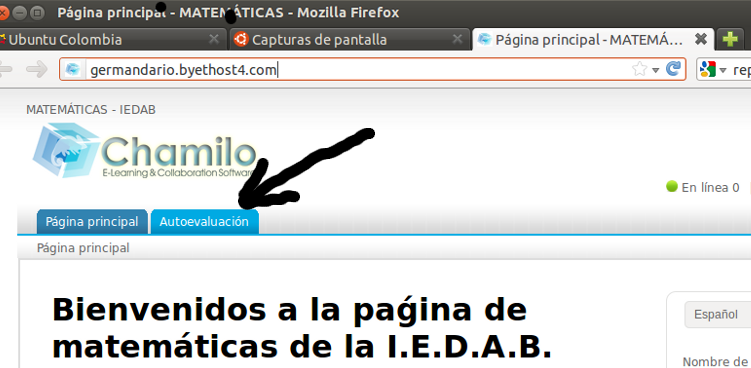
\includegraphics[scale=.35]{Images/Captura01.png} 
\end{center}
\end{frame}
\begin{frame}{Evidencias del funcionamiento de la plataforma}
\begin{center}
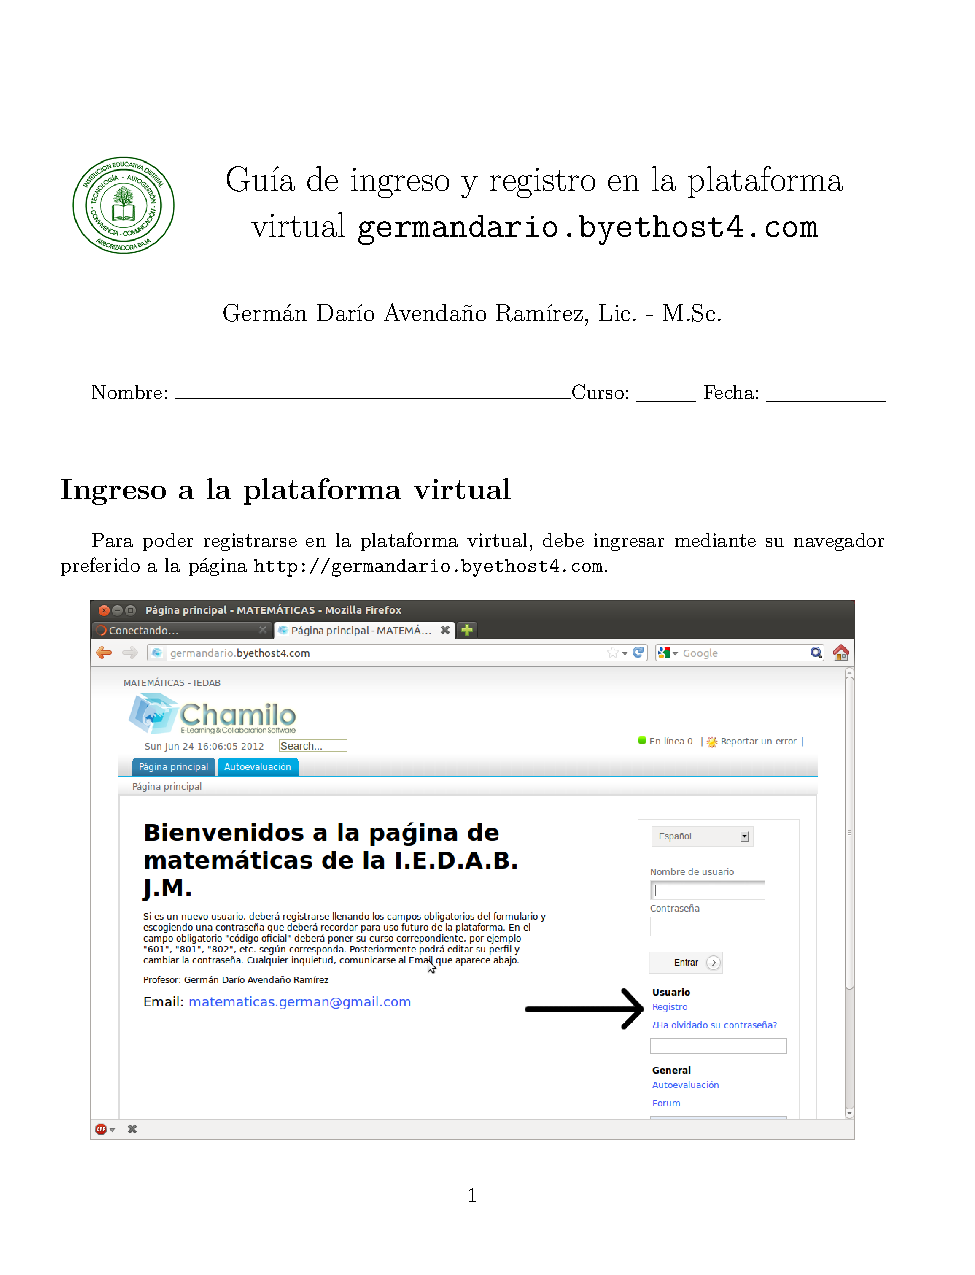
\includegraphics[scale=.4,trim=1cm 2.75cm 1cm 2.75cm,clip]{Images/GuiaIngresPlataforma1.pdf} 
\end{center}\end{frame}
\begin{frame}
\begin{center}
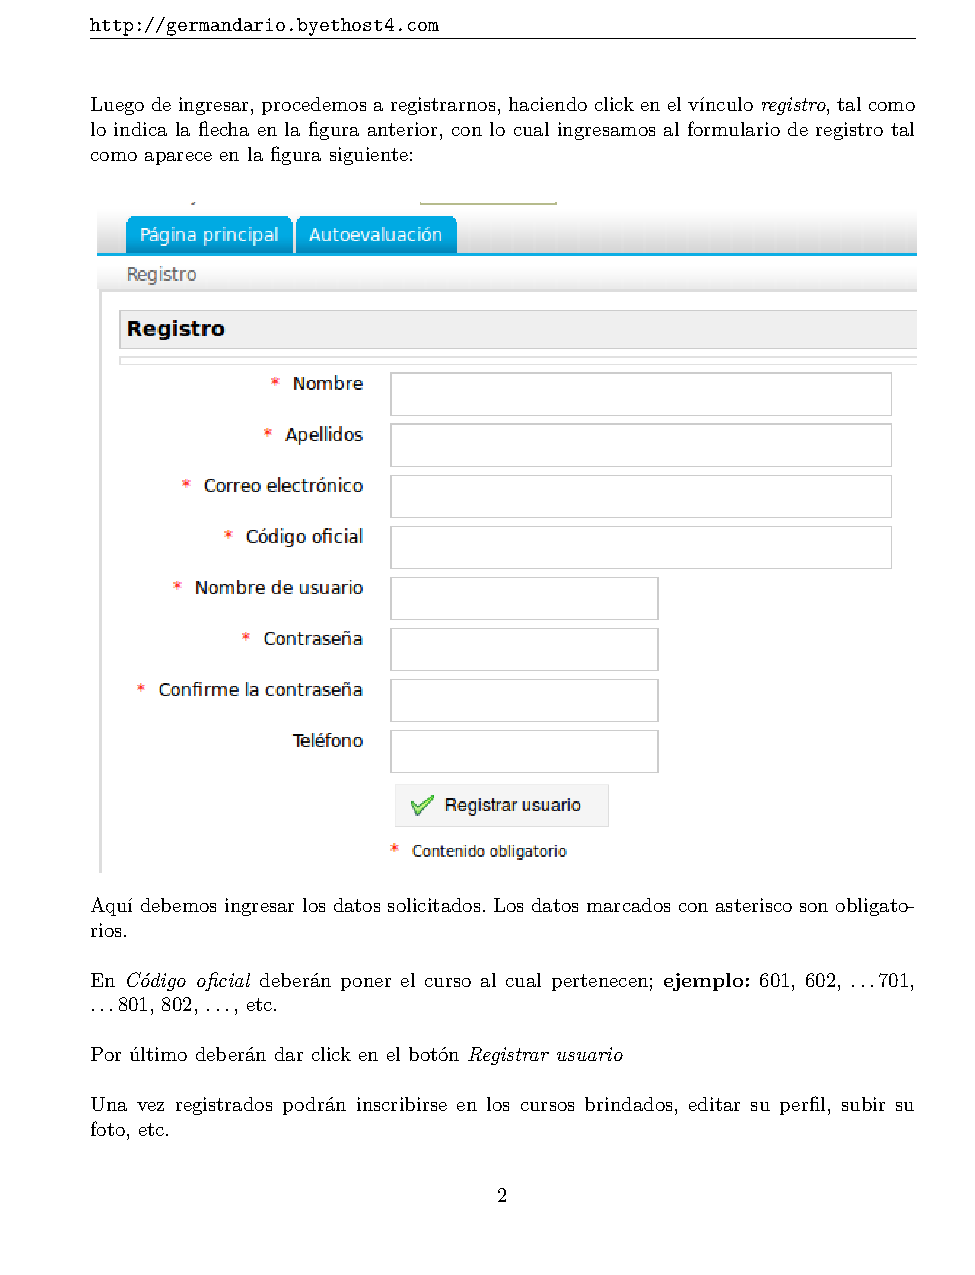
\includegraphics[scale=.375,trim=1cm 2.25cm 1cm 1.7cm,clip]{Images/GuiaIngresPlataforma2.pdf}
\end{center}
\end{frame}
\section{FASE DE ENTRADA}
\begin{frame}{FASE DE ENTRADA}
Aquí se presentan las siguientes etapas:
\begin{itemize}
  \item Motivación\pause
  \item Contextualización \pause
  \item Exploración diagnóstica
\end{itemize}
\end{frame}

\subsection[Motivación]{Motivación}

\begin{frame}{Motivación}
  % - A title should summarize the slide in an understandable fashion
  %   for anyone how does not follow everything on the slide itself.
Aquí se sugiere presentar una situación problemática que sea factible de solucionar en el desarrollo de la unidad. Debe ser,
\begin{itemize}
  \item Lo suficientemente compleja para que pueda solucionarse a través del desarrollo de la unidad
    \pause
  \item Con cierto grado de sencillez que permita su desarrollo y no lleve a frustración.
\end{itemize}
\end{frame}

\begin{frame}{Ejemplo}{Creación de plataforma virtual}
\begin{itemize}
  \item Como maestro preocupado por el proceso de enseñanza-aprendizaje en tiempos ``modernos'' ¿no le gustaría diseñar su propia plataforma e-learning?
  \pause
  \item Esto es posible gracias a una gran comunidad que promueve el uso del ``software libre'' a nivel mundial.
\end{itemize}
\end{frame}
\subsection{Contextualización}
\begin{frame}{Contextualización: Breve historia}
Se puede recurrir a la historia
\begin{itemize}
\item GNU es un acrónimo recursivo que quiere decir GNU Is Not Unix (en español se pronuncia ``ñu'').
\pause
\item Unix es un sistema operativo no libre. GNU se creó para ser compatible con Unix.
\pause
\item La idea original fue crear un sistema operativo \%100 libre.
\pause
\item Para asegurar que el software GNU permaneciera libre para que todos los usuarios pudieran ``ejecutarlo, copiarlo, modificarlo y distribuirlo'', el proyecto debía ser liberado bajo una licencia diseñada para garantizar esos derechos al tiempo que evitase restricciones posteriores de los mismos.
\end{itemize}
\end{frame}

\begin{frame}
\begin{itemize}
\item La idea se conoce en Inglés como copyleft -`izquierda de autor'- (en clara oposición a copyright -`derecho de autor'-), y está contenida en la Licencia General Pública de GNU (GPL). Aunque la acepción más reconocida de copyleft es ``copia permitida''.
\begin{figure}
  \begin{center}
    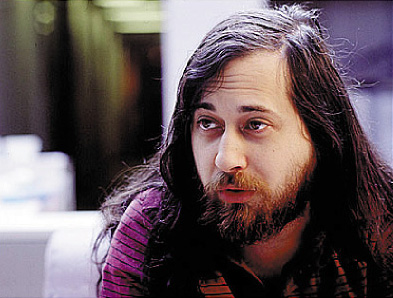
\includegraphics[scale=0.35]{Images/Richard_Matthew_Stallman.jpeg}
    \label{fig:richard}
    \caption{Richard Stallman iniciador del proyecto GNU}
  \end{center}
\end{figure}

\end{itemize}
\end{frame}

\begin{frame}
  \begin{itemize}
  \item En 1985, Stallman creó la Free Software Foundation (FSF o Fundación para el Software Libre) para proveer soportes logísticos, legales y financieros al proyecto GNU. La FSF también contrató programadores para contribuir a GNU, aunque una porción sustancial del desarrollo fue (y continúa siendo) producida por voluntarios. A medida que GNU ganaba renombre, negocios interesados comenzaron a contribuir al desarrollo o comercialización de productos GNU y el correspondiente soporte técnico. El más prominente y exitoso de ellos fue Cygnus Solutions, ahora parte de Red Hat.
    \end{itemize}
 \end{frame}
 
 \begin{frame}
 \begin{itemize}
  \item En 1990, el sistema GNU ya tenía un editor de texto llamado Emacs, un exitoso compilador (GCC), y la mayor parte de las bibliotecas y utilidades que componen un sistema operativo UNIX típico. Pero faltaba un componente clave llamado núcleo (kernel en inglés).
\pause
  \item En 1991 un estudiante finlandés crea lo que falta a GNU para que fuera un sistema operativo completamente libre. Linus Torvald crea el kernel (núcleo) ``Linux''
\end{itemize}
\end{frame}

\subsection{Exploración diagnóstica}
\begin{frame}{¿Qué sabemos?}
Aquí se hace una exploración de los saberes que posee el estudiante
\begin{itemize}
  \item  ¿Qué es el software libre?
  \item ¿Libre significa gratuito?
  \item Nombre al menos un programa que usted considere que sea software libre
  \item ¿Que es una distribución Gnu/Linux?
\end{itemize}
\end{frame}

\section{FASE DE INTRODUCCIÓN AL TEMA}
\subsection{Marco de referencia}
\begin{frame}{MARCO DE REFERENCIA}
  Aquí se presentan:
  \begin{enumerate}
    \item Los datos y hechos relevantes.\pause
    \item El marco conceptual propiamente dicho
  \end{enumerate}
\end{frame}

\begin{frame}{Qué es software libre}
  \begin{itemize}
    \item El `software libre' es una cuestión de libertad, no de precio. Para entender el concepto, debería pensar en `libre' como en `libre expresión', no como en `barra libre'.\pause
    \item El software libre es una cuestión de la libertad de los usuarios de ejecutar, copiar, distribuir, estudiar, cambiar y mejorar el software. Más precisamente, significa que los usuarios de programas tienen las cuatro libertades esenciales.
  \end{itemize}
  \end{frame}

\begin{frame}{Las cuatro libertades esenciales}
\begin{itemize}
  \item[0] La libertad de ejecutar el programa, para cualquier propósito (libertad 0)
  \pause
  \item[1] La libertad de estudiar cómo trabaja el programa, y cambiarlo para que haga lo que usted quiera. El acceso al código fuente es una condición necesaria para ello. (libertad 1)
  \pause
  \item[2] La libertad de redistribuir copias para que pueda ayudar al prójimo.
  \pause
  \item[3] La libertad de distribuir copias de sus versiones modificadas a terceros. Si lo hace, puede dar a toda la comunidad una oportunidad de beneficiarse de sus cambios. El acceso al código fuente es una condición necesaria para ello.
  \end{itemize}
\end{frame}

\section[FASE DE ELABORACIÓN]{FASE DE ELABORACIÓN}
\subsection{Estrategias de aprendizaje}
\begin{frame}{FASE DE ELABORACIÓN}
  Aquí se diseñan y se presentan las estrategias de aprendizaje de habilidades básicas y operaciones mentales, así como de los contenidos procedimentales y actitudinales. Inicialmente se deben trabajar las funciones cognitivas y las operaciones mentales como:\pause
  \begin{itemize}
    \item Identificación\pause
    \item Comparación\pause
    \item Clasificación\pause
    \item Codificación y descodificación\pause
    \item Análisis - síntesis
  \end{itemize}
\end{frame}

\section{FASE DE SALIDA}

\begin{frame}{FASE DE SALIDA}
\begin{itemize}
  \item Aquí, las estrategias de aprendizaje conllevan al desarrollo del pensamiento divergente convergente, que tiene que ver con que el estudiante sea capaz de solucionar problemas con base en la teoría. Se insiste en que se ``propone'' con base en el conocimiento.\pause
  \item Se debe terminar de solucionar el problema planteado en la motivación.\href{file:///home/german/Descargas/index.php.html}{(\underline{Creación de plataforma e-learning})}
  \end{itemize}
\end{frame}
\subsection{Creación de una plataforma virtual lms}
\begin{frame}{Creación de una plataforma virtual lms}
\begin{itemize}
\item Para la creación de la plataforma virtual, se requiere de un servidor preferiblemente LAMP (con núcleo Linux) que ofrezca
\begin{itemize}
\item Linux (kernel 3.0 o superior recomendado) en cualquier distribución (Debian y Ubuntu recomendadas)
\item Apache (versión 2.2 o superior) o Nginx con PHP5­FPM
\item MySQL (versión 5.1 o superior) o MariaDB versiones 5 o 10
\item PHP5 (versión 5.4 o superior, 5.5 o superior recomendadas por eficiencia)
\end{itemize}
 Un servidor con estas características se puede conseguir por un costo desde \$100.000 anuales.
\end{itemize}
\end{frame}
\section*{Bibliografía}
\begin{frame}[allowframebreaks]
  \frametitle<presentation>{Referencias}
    
  \begin{thebibliography}{10}
    
    \bibitem{gnu}
    \url{www.gnu.org}

  \bibitem{tdlp}\url{tdlp.org}
  
  \bibitem{fsf}\url{http://www.fsf.org/}
  
  \bibitem{sources}\url{sourceforge.net}
  
\bibitem{chamilo}\url{https://chamilo.org/es/}  
  
  \bibitem{coll}COLL, César
  \newblock {\em Los contenidos en la reforma}
  \newblock Ediciones Santillana S.A.
  \newblock 1994
  \end{thebibliography}
\end{frame}

\end{document}
